\chapter{p3 = 45 (1 graphs)}
\newpage\begin{figure}
  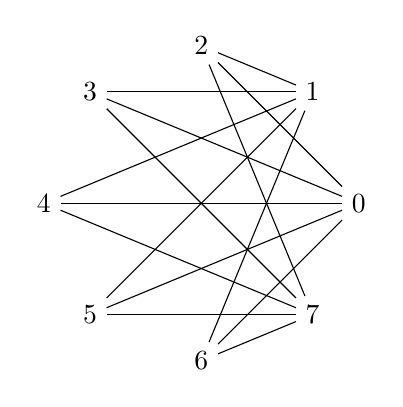
\begin{tikzpicture}
      \draw
        (0.0:2) node (0){0}
        (45.0:2) node (1){1}
        (90.0:2) node (2){2}
        (135.0:2) node (3){3}
        (180.0:2) node (4){4}
        (225.0:2) node (5){5}
        (270.0:2) node (6){6}
        (315.0:2) node (7){7};
      \begin{scope}[-]
        \draw (0) to (2);
        \draw (0) to (3);
        \draw (0) to (4);
        \draw (0) to (5);
        \draw (0) to (6);
        \draw (1) to (2);
        \draw (1) to (3);
        \draw (1) to (4);
        \draw (1) to (5);
        \draw (1) to (6);
        \draw (2) to (7);
        \draw (3) to (7);
        \draw (4) to (7);
        \draw (5) to (7);
        \draw (6) to (7);
      \end{scope}
    \end{tikzpicture}
\end{figure}
\begin{itemize}
\item signature: 0111110111110000010001001011
\item g: Graph with 8 nodes and 15 edges
\item order: 8
\item size: 15
\item max degree: 5
\item degrees: 3,3,3,3,3,5,5,5
\item is tree: 0
\item is bipartite: 1
\item has bridge: 0
\item is chordal: 0
\item is complete: 0
\item min cycle basis weight: 32
\item min cycle basis size: 8
\item diameter: 2
\item radius: 2
\item is eulerian: 0
\item is planar: 0
\item number of faces: 9
\item is regular: 0
\item p3: 45
\item p4: None
\item property hash: fea993e397be8dc464090a59c1f775eacccb5cbba68b54d5d828610b89469204
\end{itemize}
\newpage
